\documentclass[11pt]{article}

\usepackage[margin=1in]{geometry}
\usepackage{amsmath,amssymb,amsthm}
\usepackage{booktabs}
\usepackage{graphicx}
\usepackage{float}
\usepackage{placeins}
\usepackage{wrapfig}
\IfFileExists{microtype.sty}{\usepackage{microtype}}{}
\usepackage{xcolor}
\usepackage[numbers,sort&compress]{natbib}
\usepackage{hyperref}

\hypersetup{
  colorlinks=true,
  linkcolor=blue!55!black,
  citecolor=blue!55!black,
  urlcolor=blue!55!black
}

\newtheorem{theorem}{Theorem}
\newtheorem{lemma}[theorem]{Lemma}
\newtheorem{proposition}[theorem]{Proposition}
\newtheorem{corollary}[theorem]{Corollary}
\theoremstyle{remark}
\newtheorem{remark}[theorem]{Remark}
\newfloat{algorithm}{tbp}{loa}
\floatname{algorithm}{Algorithm}

\newcommand{\E}{\mathbb{E}}
\newcommand{\Cov}{\operatorname{Cov}}
\newcommand{\Var}{\operatorname{Var}}

\title{\bf Rethinking Policy Optimization with Gradient Estimators}
\author{Dongkyu Derek Cho, Thomas Voice}
\date{}

\begin{document}
\maketitle

\begin{abstract}
Clipping is widely used in policy optimization to stabilize learning under policy mismatch. In large language model post-training, however, importance-weighted updates with weak or no clipping can learn effectively for many iterations before abruptly becoming unstable, a behavior not explained by population-level policy-deviation arguments alone. We show that this transition can be understood as a finite-sample gradient-estimation problem. By expressing the off-policy policy gradient as an importance-weighted mean estimator, we connect its estimation error to effective sample size (ESS) and establish how this error determines finite-sample policy improvement. This analysis further reveals when the variance reduction from truncation or clipping outweighs the useful gradient signal it removes, motivating a simple ESS-conditioned rule that activates clipping only after estimator reliability deteriorates. Controlled experiments and large-scale LLM training show that ESS predicts this reliability transition and that ESS-conditioned clipping improves stability and learning efficiency across model scales and objectives.
\end{abstract}

\section{Introduction}
Reinforcement learning has become central to the post-training of large language
models (LLMs) \citep{bai2022hh,shao2024deepseekmath,yu2025dapo}. In scalable
training systems, policy optimization is often effectively off-policy: a rollout
policy generates responses, while a trainer reuses the collected data for one or
more gradient updates. Consequently, the current policy need not coincide with
the policy that generated the data \citep{qi2026dppo}. This mismatch makes it
important to control how far policy optimization moves from the rollout policy.

Controlling such policy deviation has long been a central principle in policy
optimization. Trust Region Policy Optimization (TRPO) formalizes this principle
through population-level policy improvement guarantees, while Proximal Policy
Optimization (PPO) provides a simple and scalable approximation through
ratio-based clipping \citep{schulman2015trpo,schulman2017ppo}. PPO-style
objectives, including GRPO, inherit this intuition by clipping or masking updates
when sampled likelihood ratios move too far from one
\citep{shao2024deepseekmath}. The resulting theoretical picture is clear at the population level: if population gradient estimators are available, keeping the updated policy sufficiently close to the rollout policy controls the error of the surrogate objective and thereby protects policy improvement.

LLM training, however, presents a striking tension with this population-level view. Empirically, permissive estimators, including truncated importance sampling (TIS) with
large caps or even unclipped updates, can remain stable and learn considerably faster. Yet this success need not persist. Figure~\ref{fig:llm-motivation} illustrates this phenomenon: TIS with caps 3 and 5 improves steadily for many
updates before abruptly collapsing. The same update rule can therefore be highly
effective for a long period and suddenly become unreliable. This raises the
central question of this paper: \emph{when does a permissive policy-gradient
estimator cease to provide a reliable update?}

\begin{figure}[htbp]
  \centering
  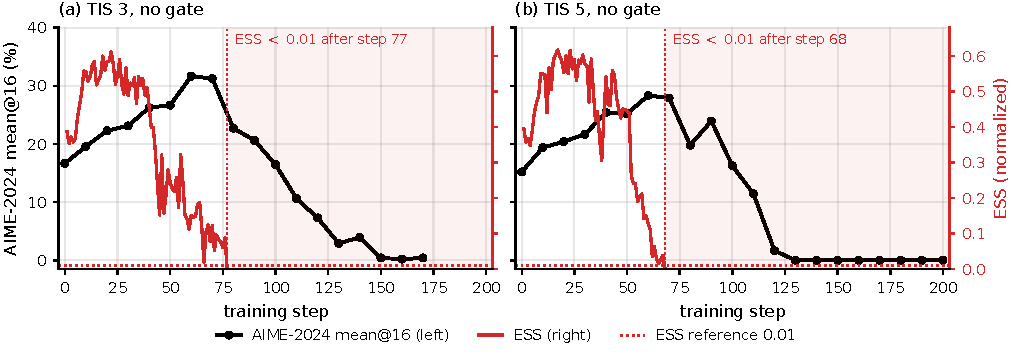
\includegraphics[width=0.9\linewidth]{figures_mains/motivation/overall.pdf}
  \caption{Delayed failure under permissive TIS updates on Qwen3-30B-A3B.
  TIS with caps 3 and 5 improves AIME-2024 mean@16 for many updates before
  effective sample size (ESS) deteriorates and performance subsequently
  collapses. The delayed transition motivates our central question: when does a
  finite rollout cease to support a reliable policy-gradient update?}
  \label{fig:llm-motivation}
\end{figure}

Classical trust-region theory explains why moving too far from the rollout policy
can be unsafe \citep{schulman2015trpo,schulman2017ppo,qi2026dppo}. It does not,
however, explain the delayed transition in Figure~\ref{fig:llm-motivation},
where failure follows many apparently successful updates rather than a single
conspicuous policy shift. Repeated updates can progressively concentrate
complete-trajectory importance weights, reducing the effective support provided
by a finite rollout even when the empirical objective is constructed from
factorwise coefficients. A population-level bound controls policy deviation,
but it does not characterize whether the available rollout still contains
enough effective information to estimate the next update reliably. The relevant
question is therefore not only \emph{how far the policy has moved}, but also
\emph{whether the finite rollout still supports a reliable gradient estimate}.

In this paper, we resolve this tension by shifting the analysis from
population-level policy deviation to finite-sample update reliability. We show
that the reliability of the policy-gradient estimator plays a central role in
determining whether an empirical update translates into policy improvement.
This perspective recasts clipping as a form of estimator control: permissive
estimators can preserve more of the learning signal when the rollout provides
sufficient effective support, whereas controlling the estimator becomes
increasingly valuable as that support deteriorates. We make this connection
explicit through effective sample size (ESS), which quantifies the concentration
of the importance weights underlying the finite-sample estimator. We then
validate this prediction empirically and use it to derive a simple optimization
rule that preserves permissive updates while they remain reliable and
intervenes when the rollout ceases to support them.

%In this work, we develop a finite-sample perspective on policy optimization that explains when permissive updates remain reliable and when stronger control becomes necessary. 

Our contributions are threefold. \textbf{Finite-Sample Policy Improvement:} We derive a policy-improvement analysis that explicitly accounts for the reliability of the empirical gradient estimator, complementing the population-level view of policy deviation with the statistical adequacy of the available rollout. \textbf{Estimator Reliability and ESS:} We interpret clipping and truncation as forms of estimator control and establish a direct connection between gradient-estimator reliability and effective sample size (ESS), explaining why permissive updates can learn rapidly when effective support is sufficient but become unstable as importance weights concentrate. \textbf{Reliability-Aware Optimization:} Guided by this analysis, we propose a simple optimization rule that preserves permissive updates while the rollout remains reliable and increases control only when reliability deteriorates. Controlled simulations and large-scale LLM reasoning experiments validate these predictions and demonstrate an improved stability-learning tradeoff over fixed clipping strategies.

\section{Related work}

%\paragraph{Trust-region and proximal policy optimization.}

Trust-region methods control policy deviation to obtain monotonic-improvement guarantees, while PPO replaces the explicit trust-region constraint with a ratio-clipped surrogate that is easier to optimize at scale
\citep{schulman2015trpo,schulman2017ppo}. However, recent analyses of LLM policy optimization show that the trust region alone does not determine the reliability of policy optimization. For example, recent empirical analyses reveal that less aggressive clipping thresholds \citep{yu2025dapo,park2025clipping,minimax2025m1,qi2026dppo} and even unclipped learning can be effective. Yet, existing works lack theoretical explanations.

Our analysis addresses a different source of error: the finite-sample gradient estimate used to make that update by linking the policy optimization to the importance-weighted estimation problem. Existing work in importance sampling reveals the central role of ratio moments in quantifying estimation uncertainty and applies this to the off-policy estimation problem \citep{metelli2018pois,metelli2020is}. We further extend these
two ingredients by relating importance-weight concentration to
gradient-estimation reliability and, in turn, to policy improvement \citep{pirotta2013adaptive,papini2022smoothing}.


\section{Preliminaries}
\label{sec:setting}

\subsection{Policy gradients from a fixed rollout}

\paragraph{Policy gradients.}
Let $X\sim\nu$ denote a context and let
$P_\theta(\cdot\mid X)$ be a parameterized policy. For a response or
trajectory $Y=(Y_1,\ldots,Y_T)$ with reward $R(X,Y)$, the policy objective is given as $J(\theta)
 :=
 \E_{X\sim\nu,\;Y\sim P_\theta(\cdot\mid X)}
 [R(X,Y)].$

Parameterized policy learning seeks a parameter $\theta$ that maximizes the policy objective $J(\theta)$. Policy-gradient methods learn this parameter through gradient ascent. By classical control-variate analysis and the score function identity, the policy gradient admits the following form:
\begin{equation}
 g(\theta)
 :=
 \nabla J(\theta)
 =
 \E_{P_\theta}
 \left[
 A(X,Y)
 \sum_{t=1}^T
 \nabla_\theta
 \log P_\theta(Y_t\mid X,Y_{<t})
 \right].
 \label{eq:on-policy-gradient}
\end{equation}
Here, $A(X,Y):=R(X,Y)-b(X)$ is the control-variate adjusted advantage, where the baseline $b(X)$ leaves the expected gradient unchanged while reducing its variance.

The expectation in Equation~\eqref{eq:on-policy-gradient} is taken under the current policy $P_\theta$. For efficiency, modern policy-optimization methods often rely on reusing data \citep{schulman2017ppo, schulman2015trpo}, which creates a mismatch between the current policy and the rollout policy $Q(\cdot\mid X)$. This mismatch is then accounted for by the likelihood ratio. 

Formally, define the likelihood ratio and score $ r_{\theta,t}
 :=
 \frac{P_\theta(Y_t\mid X,Y_{<t})}
      {Q(Y_t\mid X,Y_{<t})},~
 \ell_{\theta,t}
 :=
 \nabla_\theta
 \log P_\theta(Y_t\mid X,Y_{<t}).$ Given i.i.d.\ rollouts
$Z_i=(X_i,Y_i)\sim\nu(dx)Q(dy\mid x)$, $i=1,\ldots,N$, and assuming
$P_\theta(\cdot\mid X)\ll Q(\cdot\mid X)$, a change of measure rewrites the population gradient and its sample analogue under the rollout distribution:
\begin{equation}
 g(\theta)
 =
 \E_Q[W_\theta f_\theta], \qquad \widehat g_N(\theta)
 :=
 \frac1N\sum_{i=1}^N
 W_{\theta,i}f_{\theta,i},
 \label{eq:true-gradient}
\end{equation}
where $f_\theta
 :=
 A(X,Y)\sum_{t=1}^T\ell_{\theta,t}$ denotes the score and advantage contribution and $ W_\theta=
 \prod_{t=1}^T r_{\theta,t}$ becomes the complete sample likelihood ratio.
 
 Equation~\eqref{eq:true-gradient} reveals the connection between policy-gradient optimization and the importance-weighted mean-estimation problem, which is a foundational problem in statistics. The quality of the resulting policy update therefore depends on how reliably this finite importance-weighted average estimates $g(\theta)$; the update thus inherits the challenges of importance-weighted estimation.

\paragraph{Estimator choices.}
Large or highly dispersed likelihood ratios can make
gradient estimators statistically unstable. Practical
policy-gradient algorithms therefore modify the coefficients of the empirical gradient to control this behavior. To represent these modifications in a common form,
write
$\mathbf r_\theta=(r_{\theta,1},\ldots,r_{\theta,T})$ and let
$u=(u_1,\ldots,u_T)$ denote a collection of coefficient rules. Define
\begin{equation}
 \psi_\theta(u;Z)
 :=
 A(Z)\sum_{t=1}^T
 u_t(\mathbf r_\theta,A(Z))
 \ell_{\theta,t}(Z),
 \qquad
 \widehat g_N(u;\theta)
 :=
 \frac1N\sum_{i=1}^N
 \psi_\theta(u;Z_i).
 \label{eq:coefficient-rule-estimator}
\end{equation}

Setting $u_{\mathrm{IS},t}=r_{\theta,t}$ for $t=1,\ldots,T$ corresponds to the conventional IS estimator. We consider two common estimator choices in this paper: the truncated importance sampling rule (TIS)~\citep{minimax2025m1} and PPO/GRPO clipping \citep{schulman2017ppo,shao2024deepseekmath}:
\begin{equation*}
 u_{\mathrm{T},t}(\mathbf r,A)
 :=
 \min\{r_t,c\}, \qquad  u_{\mathrm{P},t}(\mathbf r,A)
 :=
 r_t
 \left[
 \mathbf 1\{A\ge0,\ r_t\le1+\epsilon\}
 +
 \mathbf 1\{A<0,\ r_t\ge1-\epsilon\}\right],
 \label{eq:tis-coefficient-rule}
\end{equation*}
TIS caps the corresponding ratio, which reduces the magnitude of a large importance coefficient while retaining the associated score contribution. On the other hand, PPO/GRPO clipping modifies the gradient in a qualitatively different way by an advantage-dependent masking
rule. Once the corresponding clipping condition is active, the selected score contribution is removed from the gradient.

\subsection{Importance-weight concentration and effective sample size}


Despite the central role of finite-sample gradient reliability in policy
optimization, relatively few works directly connect this reliability to the
statistical properties of the underlying gradient estimator. From the
estimator perspective developed above, however, this question can be studied
through the theory of importance-weighted mean estimation, whose finite-sample
behavior has been extensively studied in statistics. A key quantity in this
literature is the dispersion of the likelihood weights, which can be characterized through normalized effective sample size (ESS)
\citep{metelli2018pois,metelli2020is}. \begin{wrapfigure}[12]{r}{0.3\textwidth}
  \vspace{-0.6\baselineskip}
  \centering
  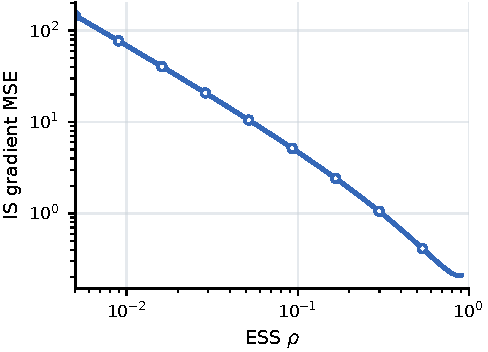
\includegraphics[width=0.85\linewidth]{figures/gaussian_is_mse.pdf}
  \caption{Exact IS gradient MSE as a function of ESS $\rho$ in the Gaussian bandit.}
  \label{fig:gaussian-is-mse}
  \vspace{-0.4\baselineskip}
\end{wrapfigure}
In our population setting, normalized
ESS can be written as
\citep{renyi1961entropy,vanerven2014renyi,metelli2018pois,metelli2020is}:



\begin{equation}
 \rho_\theta
 =
 \frac{1}{\E_Q[(W_\theta-1)^2]+1}.
 \label{eq:ess-ratio-dispersion}
\end{equation}

A low ESS therefore indicates greater dispersion of the population likelihood ratios and suggests greater finite-sample variability in importance-weighted estimation. To illustrate, we use Figure~\ref{fig:gaussian-is-mse} in the Gaussian policy optimization example in Section~\ref{sec:gaussian-example}. Here, lower ESS worsens the gradient estimator MSE. Intuitively, this further suggests that ESS provides the desired connection to reliable policy updates in Figure~\ref{fig:llm-motivation}. When ESS approaches the observed threshold, subsequent updates become unstable and eventually collapse.


\section{Theoretical Analysis}
\label{sec:theory}

In this section, we provide the theoretical analysis of the finite sample policy improvement and the estimator reliability, along with the connection with ESS.

%The estimator formulation in Section~\ref{sec:setting} reduces policy optimization from a fixed rollout to a finite-sample gradient-estimation problem. We then specialize the result to IS, for which the estimation error admits an exact second-moment representation involving ESS. The following subsection uses this reliability characterization to compare alternative estimator choices.

\subsection{Gradient-estimator reliability and policy improvement}
\label{sec:gradient-reliability}

\paragraph{MSE and policy improvement}
We first establish how mean squared error (MSE) in the estimated gradient limits one-step policy improvement. Under the smoothness condition on the parameterized policy, one can convert an arbitrary estimator's deviation from the population gradient directly into a lower bound on policy improvement.

\begin{lemma}[A reliable gradient estimate yields policy improvement]
\label{lem:gradient-error-progress}
Let $\widehat g$ be an estimate of $g=\nabla J(\theta)$ satisfying
$\|\widehat g-g\|_2\le\varepsilon$. Suppose that $J$ is $L$-smooth along the
update segment for $L>0$, and define $ \gamma
 :=
 \frac1L
 \left(
 1-\frac{\varepsilon}{\|\widehat g\|_2}
 \right)_+,$ with $\gamma=0$ when $\widehat g=0$. Then
\begin{equation}
 J(\theta+\gamma\widehat g)-J(\theta)
 \ge
 \frac{1}{2L}
 \left(
 \|\widehat g\|_2-\varepsilon
 \right)_+^2 .
 \label{eq:gradient-error-progress}
\end{equation}
\end{lemma}

Lemma~\ref{lem:gradient-error-progress} identifies the quantity
that determines whether a finite-sample direction is useful: a positive certificate for policy optimization is obtained whenever the gradient magnitude exceeds its estimation-error radius. Note that in practice, such error radius is not known, hence requires a specific characterization that can be used in practice.

\paragraph{IS reliability through ESS.}

We show that the error can be characterized explicitly by ESS. Throughout, we condition on the preceding updates and write $W_k:=W_{\theta_k}$, $f_k:=f_{\theta_k}$,
$g_k:=g(\theta_k)$, $\widehat g_k:=\widehat g_N(\theta_k)$, and
$\rho_k:=\rho_{\theta_k}$ at update $k$. The following Lemma provides the connection with a high-probability reliability
radius and ESS.

\begin{lemma}[ESS controls IS gradient reliability]
\label{lem:rho-gradient-reliability}
Suppose $d_2(P_{\theta_k}\|Q)<\infty$ and
$\E_Q[W_k^2\|f_k\|_2^2]<\infty$ and define $M_{2,k}:=\frac{\E_Q[W_k^2\|f_k\|_2^2]}{\E_Q[W_k^2]}$. Then, for any $0<\delta\le1$,
\begin{equation}
 \Pr\left(
 \|\widehat g_k-g_k\|_2
 \le
 \sqrt{\frac{M_{2,k}}{\delta N\rho_k}}
 \right)
 \ge
 1-\delta .
 \label{eq:rho-gradient-concentration}
\end{equation}
\end{lemma}

Thus the error radius entering
Lemma~\ref{lem:gradient-error-progress} scales as
$\rho_k^{-1/2}$. Substituting this radius gives the corresponding ESS-dependent improvement guarantee.

\begin{theorem}[ESS-dependent improvement for the IS estimator]
\label{thm:permissive-reliability}
Under the conditions of Lemma~\ref{lem:rho-gradient-reliability}, suppose that
$J$ is $L_k$-smooth along the update segment. For any $0<\delta\le1$, define $\varepsilon_k(\delta)
 :=
 \sqrt{\frac{M_{2,k}}{\delta N\rho_k}},
 \quad
 \gamma_k
 :=
 \frac1{L_k}
 \left(
 1-\frac{\varepsilon_k(\delta)}
        {\|\widehat g_k\|_2}
 \right)_+ ,$ with $\gamma_k=0$ when $\widehat g_k=0$. Then, with probability at least
$1-\delta$,
\begin{equation}
 J(\theta_k+\gamma_k\widehat g_k)-J(\theta_k)
 \ge
 \frac{1}{2L_k}
 \left(
 \|\widehat g_k\|_2-\varepsilon_k(\delta)
 \right)_+^2 .
 \label{eq:permissive-reliability}
\end{equation}
\end{theorem}

The preceding results establish the complete IS reliability chain. ESS enters
the exact gradient MSE through the importance-weight second moment; this MSE
determines a high-probability error radius, which in turn controls both the
magnitude and the probability of one-step policy improvement. 
%This characterization applies to unbiased IS. Once the coefficient rule is modified, bias enters the estimation error and the estimator itself changes, which requires the comparison developed next.

\subsection{Estimator reliability and ESS-dependent crossover}
\label{sec:clipping-recovery}

We now generalize the result to the general estimators. To facilitate the analysis, consider a general coefficient rule $u$. The same reliability question
must also account for the bias introduced by modifying the estimator. Write the MSE error of the gradient estimator as $m_k(u)$. We first connect MSE to the gradient-estimator reliability.

\begin{lemma}[MSE controls gradient-estimator reliability]
\label{lem:general-mse-reliability}
For any coefficient rule $u$ with $m_k(u)<\infty$ and any
$0<\delta\le1$,
\begin{equation}
 \Pr\left(
 \|\widehat g_k(u)-g_k\|_2
 \le
 \sqrt{\frac{m_k(u)}{\delta}}
 \right)
 \ge 1-\delta .
 \label{eq:general-mse-reliability}
\end{equation}
\end{lemma}

Together with Lemma~\ref{lem:gradient-error-progress},
Lemma~\ref{lem:general-mse-reliability} shows that smaller MSE yields a
tighter high-probability policy-improvement guarantee. Estimator selection,
however, is not equivalent to MSE minimization. A rule may reduce its MSE by
suppressing gradient contributions that are themselves useful for policy
improvement. The resulting optimization tradeoff is captured by the following
certificate.

\begin{theorem}[MSE form of the policy-improvement certificate]
\label{thm:fixed-step-certificate}
Suppose that $J$ is $L_k$-smooth on every update segment generated by $u$
almost surely and that
$\E\|\widehat g_k(u)\|_2^2<\infty$. For any $\eta_k>0$,
\begin{equation}
 \E\!\left[
 J(\theta_k+\eta_k\widehat g_k(u))-J(\theta_k)
 \right]
 \ge
 B_k(u;\eta_k),
 \label{eq:full-token-rule-progress}
\end{equation}
where
\begin{equation}
 B_k(u;\eta_k)
 =
 \frac{\eta_k}{2}\|g_k\|_2^2
 -
 \frac{\eta_k}{2}m_k(u)
 +
 \frac{\eta_k}{2}(1-L_k\eta_k)
 \E\|\widehat g_k(u)\|_2^2 .
 \label{eq:certificate-mse-form}
\end{equation}
\end{theorem}

Equation~\eqref{eq:certificate-mse-form} places estimator reliability and
policy improvement in the same expression. Lower MSE strengthens the
certificate, while coefficient control can simultaneously reduce the
magnitude of the update. The preferred estimator therefore depends on whether
the reduction in estimation error is large enough to compensate for the useful update removed by the modification. Such a preferred estimator can be determined by comparing the lower bounds on policy improvement.

\begin{corollary}[Estimator crossover]
\label{cor:certificate-crossover}
Let $u$ and $v$ use the same step size $0<\eta_k\le1/L_k$. Then
\begin{equation}
 B_k(u;\eta_k)>B_k(v;\eta_k)
 \quad\Longleftrightarrow\quad
 m_k(v)-m_k(u)
 >
 (1-L_k\eta_k)
 \left\{
 \E\|\widehat g_k(v)\|_2^2
 -
 \E\|\widehat g_k(u)\|_2^2
 \right\}.
 \label{eq:general-estimator-crossover}
\end{equation}
\end{corollary}

Corollary~\ref{cor:certificate-crossover} shows that estimator selection is
determined by a tradeoff between the reduction in estimation error and the
corresponding change in update magnitude. Evaluating this crossover directly,
however, requires population MSEs and second moments. The results of Section~4.1 allow its contribution to be expressed in terms of ESS, yielding the following specialization.

\begin{proposition}[ESS-dependent estimator crossover]
\label{prop:ess-estimator-crossover}
Let $u$ be an alternative coefficient rule and suppose
$0<\eta_k\le1/L_k$. Then $u$ has a stronger certificate than IS if and only if
\begin{equation}
 \frac{L_k\eta_k M_{2,k}}{N\rho_k}
 >
 m_k(u)
 -
 (1-L_k\eta_k)
 \E\|\widehat g_k(u)\|_2^2
 +
 \left(
 1-L_k\eta_k+\frac{L_k\eta_k}{N}
 \right)
 \|g_k\|_2^2 .
 \label{eq:ess-estimator-crossover}
\end{equation}
\end{proposition}

Proposition~\ref{prop:ess-estimator-crossover} isolates the role of ESS in the crossover. Decreasing ESS makes the inequality easier to satisfy and therefore shifts the comparison toward estimator control, favoring the conservative updates such as clipping. 

%The precise crossover remains estimator dependent, which allows truncation and clipping to become preferable at different ESS levels.

%All dependence of the IS certificate on importance-weight concentration appears through $1/\rho_k$ on the left-hand side, whereas the right-hand side collects the corresponding MSE and second-moment terms of the alternative estimator. 

\paragraph{TIS under rare truncation.}

TIS changes the estimator only on ratios exceeding its cap. Let $u_{\mathrm T}^{(\infty)}$ denote the corresponding untruncated factorwise importance-weighted rule, $u_{\mathrm T,t}^{(\infty)}=r_t$. The following rule demonstrates the similarity between TIS and IS estimators. 
\begin{proposition}[Truncation preserves the importance-weighted certificate]
\label{prop:tis-close}
Suppose that the conditional second moment of
$A(r_{\theta_k,t}-c)_+\ell_{\theta_k,t}$ on
$\{r_{\theta_k,t}>c\}$ is uniformly bounded, and write $ p_{c,k}
 :=
 \frac1T\sum_{t=1}^T
 \Pr(r_{\theta_k,t}>c).$ Then, for fixed remaining
moments,
\begin{equation}
 \left|
 B_k(u_{\mathrm T};\eta_k)
 -
 B_k(u_{\mathrm T}^{(\infty)};\eta_k)
 \right|
 =
 O(\sqrt{p_{c,k}})
 \qquad\text{as }p_{c,k}\rightarrow0 .
 \label{eq:tis-close-certificate}
\end{equation}
\end{proposition}

Proposition~\ref{prop:tis-close} shows that TIS retains the improvement certificate of untruncated importance weighting when truncation affects only a small, controlled tail. PPO-style clipping makes a stronger modification, which masks the entire $r_t$-weighted contribution. It can therefore produce a larger reduction in estimator variation, but requires that reduction to compensate for a correspondingly larger change in the mean update.

Together, our analysis reveals the importance of the policy gradient reliability in policy optimization and suggests ESS as the observable reliability criterion. Further, Theorem~\ref{thm:permissive-reliability} and Proposition~\ref{prop:ess-estimator-crossover} provide insight into when other estimators can be beneficial in some cases. High ESS suggests using permissive gradient estimators, and lower ESS suggests more conservative choices such as clipping, highlighting the potential benefit of stronger estimator variance control.

%give the explanation why permissive updates could fail when ESS is small. The smaller ESS implies observable ESS values correlate with the reliable policy optimization. When ESS is relatively large, the IS estimation error is small and mild truncation can preserve the resulting importance-weighted update. As ESS decreases, the growing finite-sample error of IS increases the potential benefit of stronger variance control. 


\section{Policy optimization and ESS}
In this section, we demonstrate our theoretical analysis in two settings. Here, we present our results on the Gaussian bandit and LLM trajectories.

%We first use an analytically tractable Gaussian bandit to instantiate IS reliability, estimator crossover, and one-step policy improvement. Large-model trajectories then show how observed ESS evolves around delayed optimization failure.

\subsection{Policy optimization in a Gaussian bandit}
\label{sec:gaussian-example}
We consider Gaussian policies with quadratic rewards, which admit closed-form population gradients and estimator moments. We first test whether ESS predicts when IS loses finite-sample reliability and then compare policy-improvement gains along a path of varying ESS. Appendix~\ref{app:gaussian} gives the calculations and protocol.

\begin{figure}[htbp]
  \centering
  % Original: 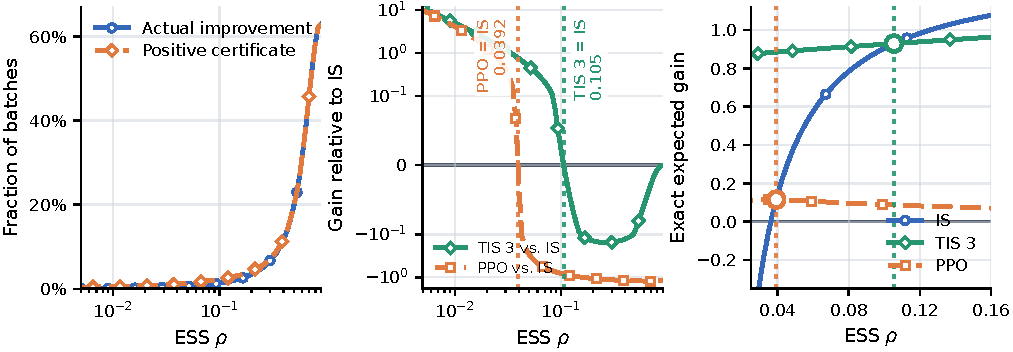
\includegraphics[width=0.9\linewidth]{figures/gaussian_policy_comparison.pdf}
  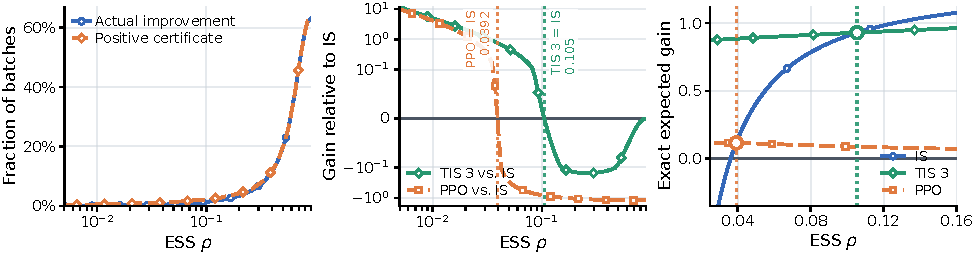
\includegraphics[width=0.9\linewidth]{figures/gaussian_policy_comparison_compact.pdf}
  \caption{Gaussian-bandit reliability and estimator comparison. From left
  to right: positive certificates and actual positive improvement under the
  adaptive IS step; exact expected gain of TIS-3 and PPO relative to IS; and
  exact expected gain near the pairwise crossovers. Vertical lines and open
  markers identify the intersections.}
  \label{fig:gaussian-policy-comparison}
\end{figure}

\paragraph{ESS predicts reliability and policy improvement}
The left plot in Figure~\ref{fig:gaussian-policy-comparison} illustrates how
estimator reliability translates into policy improvement. Across the full ESS
path, the probability of actual improvement tracks the probability of a
positive certificate with a maximum gap of only $0.00891$. As support
contracts, both probabilities fall together. ESS therefore identifies when a
reliable IS update is available, but this first stage leaves one question
open: which controlled estimator should be used after IS loses its advantage?

\paragraph{ESS determines estimator-choice criterion}
Figure~\ref{fig:gaussian-policy-comparison} then demonstrates the estimator-selection
criterion in Corollary~\ref{cor:certificate-crossover}.
The center plot gives the resulting expected-gain
difference relative to IS. TIS-3 has the lowest MSE throughout the path, yet
IS retains more useful gradient alignment and therefore has the larger gain
at high ESS. As ESS falls, the variance reduction from truncation becomes
decisive, and TIS-3 overtakes IS at $\rho=0.105$. PPO removes still more
alignment, so it crosses IS only at $\rho=0.0392$. The right plot makes both
transitions visible as intersections of the exact policy-improvement curves.
The resulting upper envelope selects IS in the high-support regime and TIS-3
in the low-support regime, exactly as predicted by the gain criterion.

\subsection{Policy optimization in large language models}
\label{sec:llm-reliability}

\begin{figure}[htbp]
  \centering
  % Original: 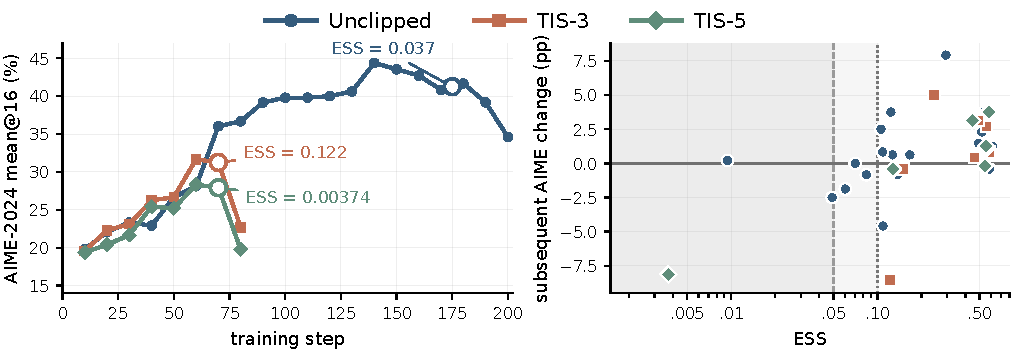
\includegraphics[width=0.8\linewidth]{figures_mains/motivation/ess_reliability_collapse_ess_unclipped_combine.pdf}
  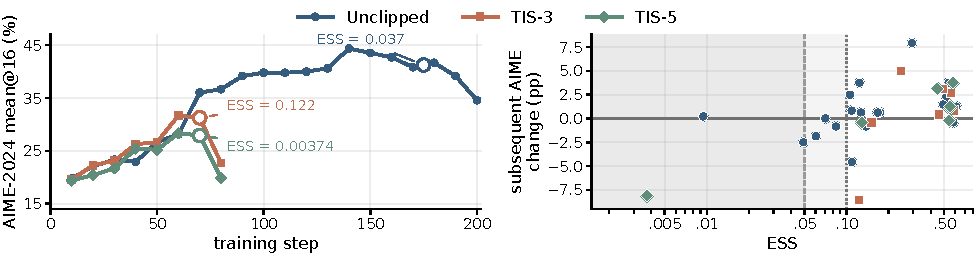
\includegraphics[width=0.8\linewidth]{figures_mains/motivation/ess_reliability_collapse_compact.pdf}
  \caption{
  Left: AIME-2024 mean@16 along an unclipped trajectory and TIS with caps
  3 and 5. Annotations report ESS at the onset of the
  sustained performance decline. Right: each point pairs ESS at an evaluation checkpoint with the
  change in AIME-2024 mean@16 over the following ten updates. The shaded
  regions indicate ESS below $0.1$ and $0.05$. Lower ESS is associated with
  substantially weaker and less reliable subsequent improvement.}
  \label{fig:ess-local-improvement}
\end{figure}
We now examine whether the same finite-sample mechanism is
visible during large-model optimization. We consider three Qwen3-30B-A3B trajectories, consisting of an unclipped update and TIS with caps 3 and 5, and evaluate all trajectories on AIME-2024 using mean@16.

The left panel of Figure~\ref{fig:ess-local-improvement} places ESS within the training dynamics. The right panel tests the theoretical prediction more directly. At each evaluation checkpoint, we pair the current ESS with the change in AIME-2024
mean@16 over the following ten updates. The resulting pattern shows a clear change in update reliability as ESS decreases. Low ESS identifies a regime in which continued
importance-weighted updates are substantially less likely to produce reliable improvement. This behavior is the effect characterized in Section~\ref{sec:theory}, where decreasing ESS enlarges the gradient-error radius through the factor $\rho_k^{-1/2}$ and consequently weakens the corresponding policy-improvement certificate. %Thus, the delayed failure observed in the introduction occurs after a substantial deterioration in the importance-weight distribution, even though the precise ESS value at which degradation begins differs across trajectories. 

%All three importance-weighted updates improve substantially during the early stage of training, but their performance eventually begins to degrade. At the onset of the sustained decline, all three methods exhibit low ESS. 

%The large-model trajectories exhibit the same optimization consequence: as ESS deteriorates, subsequent improvement becomes less reliable. This observation motivates the optimization rule studied next: retain the importance-weighted update while its reliability remains high, and introduce clipping when ESS indicates that additional estimator control has become valuable.

\section{ESS-conditioned policy optimization}
\label{sec:ess-conditioned-optimization}

%The preceding experiments show that decreasing ESS accompanies a loss of reliable subsequent improvement under importance-weighted updates. 

\begin{figure}[htbp]
  \centering
  % Original: 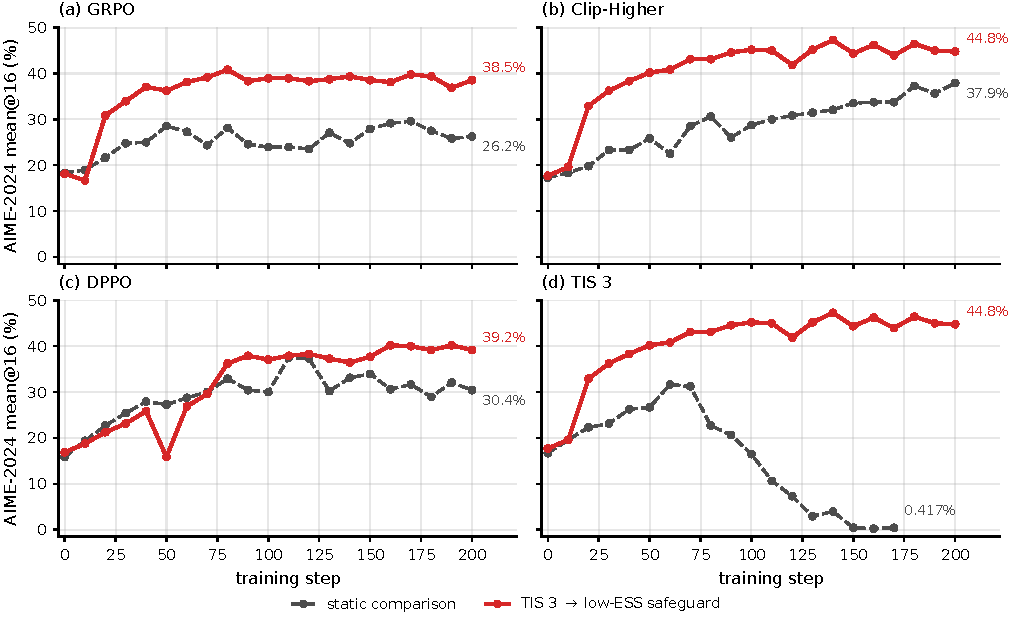
\includegraphics[width=0.8\linewidth]{figures_mains/result/q30ba3b/curves/overall.pdf}
  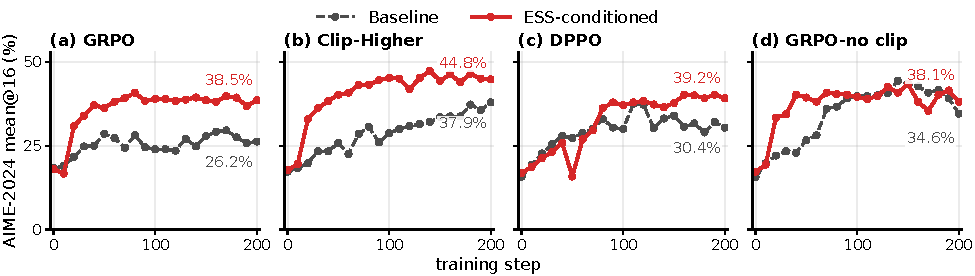
\includegraphics[width=\linewidth]
  {figures_mains/result/q30ba3b/curves/overall_with_noclip_compact.pdf}
  \caption{Qwen3-30B-A3B math RLVR results. Dashed curves
  correspond to the baseline methods. Solid curves begin with TIS-3 in (a), (b), and (c), or an unclipped update in (d), and switch to the corresponding clipped update when ESS falls below $0.1$. (a) GRPO clipping. (b) Clip-Higher. (c) DPPO. (d) GRPO-no clip.} %End labels report the final observed AIME-2024 mean@16.}
  \label{fig:llm-main}
  \label{fig:llm-noclip-gate}
\end{figure}

\begin{wrapfigure}[13]{R}{0.36\textwidth}
  \vspace{-0.7\baselineskip}
  \centering
  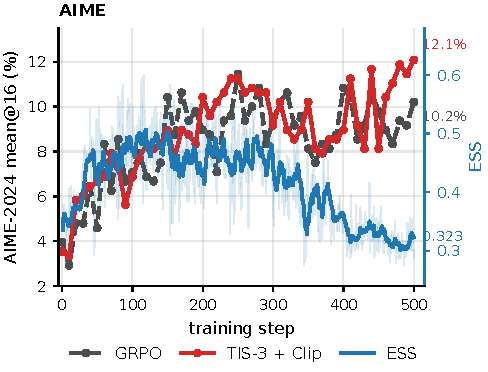
\includegraphics[width=0.9\linewidth]{figures_mains/result/q17b/overall.pdf}
  \caption{ Qwen3-1.7B results over extended training. Dashed black: GRPO, Red: ESS-cond (red). The blue line represents ESS for ESS-cond.}
  \label{fig:llm-rlhf-transfer}
  \vspace{-0.6\baselineskip}
\end{wrapfigure}
In this section, we now extend our theoretical analysis to an optimization rule. Based on this observation, the reliability signal can be used in optimization to determine the \emph{clipping timing}. While ESS remains above a fixed threshold, we retain importance-weighted updates and activate clipping for conservative updates.

%ask whether this reliability signal can be used to optimization. Rather than applying clipping throughout training, we retain the importance-weightedupdate while ESS remains above a fixed threshold and activate clipping once ESS falls below it.



\subsection{Update rule and protocol}

% Original standalone figure, now displayed in panel (d) above.
% \begin{wrapfigure}{r}{0.35\textwidth}
%   \vspace{-0.7\baselineskip}
%   \centering
%   \includegraphics[width=0.95\linewidth]
%   {figures_mains/result/q30ba3b/noclip/overall.pdf}
%   \caption{Qwen3-30B-A3B math RLVR with an unclipped update. Dashed: unclipped
%   throughout. Solid: ESS-conditioned clipping.}
%   \label{fig:llm-noclip-gate}
%   \vspace{-0.6\baselineskip}
% \end{wrapfigure}

Let $\widehat g_{\mathrm{IW}}$ denote the importance-weighted update such as IS or TIS, and $\widehat g_{\mathrm{clip}}$ a prespecified clipped update. Given an ESS threshold $\tau$, we use the following gradient estimator:
\begin{equation}
  \widehat g_{\mathrm{ESS}}
  =
  \begin{cases}
    \widehat g_{\mathrm{IW}},
      & \widehat\rho \ge \tau,\\
    \widehat g_{\mathrm{clip}},
      & \widehat\rho < \tau,
  \end{cases}
  \label{eq:llm-gate}
\end{equation}
%ESS therefore determines when clipping is introduced, while the clipping rule determines how the update is modified thereafter. 
where we use $\tau=0.1$ in the experiments.

In the main experiments, we investigate the configurations that demonstrated failure modes, and see whether our intervention rule yields reliable updates. We consider the following on Qwen3-30B-A3B base models: (1) TIS-3 updates with GRPO clipping \citep{shao2024deepseekmath}, (2) TIS-3 updates with Clip-Higher \citep{yu2025dapo}, (3) TIS-3 updates with DPPO \citep{qi2026dppo}, (4) unclipped updates with GRPO clipping \citep{shao2024deepseekmath}. Baseline models include GRPO, GRPO with no clips, Clip-Higher, DPPO, and TIS-3 updates. Our main experiments train models for up to 200 training steps on the mathematical-reasoning data of \citet{yu2025dapo} and evaluate AIME-2024 using mean@16.

%For importance-weighted updates, we use TIS with ratio cap 3 as a default choice. At low ESS, we consider conventional GRPO clipping \citep{shao2024deepseekmath}, Clip-Higher \citep{yu2025dapo}, and DPPO \citep{qi2026dppo}. We additionally replace TIS-3 with an unclipped update totest whether the timing principle depends on truncation.

\subsection{Results}
\label{sec:llm-experiments}
The first three panels of Figure~\ref{fig:llm-main} compare ESS-conditioned optimization with static clipping across corresponding baselines. In all three cases, ESS-conditioned optimization presents stronger AIME performance and efficiency. Specifically, while TIS-3 and unclipped GRPO present instability, the ESS-conditioned optimization exhibits remarkable stability, preventing catastrophic collapses.


Figure~\ref{fig:llm-noclip-gate}(d) leaves one run
unchanged and introduces conventional clipping in the other when ESS falls below $0.1$. While the unclipped run subsequently degrades to $34.6\%$, ESS-conditioned learning retains $38.1\%$ at step 200. The timing principle therefore extends beyond the TIS-3 branch. 

Together, these panels show the empirical strength of the ESS-conditioned optimization, which supports the theoretical motivation.

\subsection{Broader Evaluation}

\paragraph{Results on Different Scales.}
We first change model scale while retaining the
mathematical-reasoning objective. Figure~\ref{fig:llm-8b-transfer} extends the recipe comparison to dense Qwen3-8B. ESS-conditioned optimization demonstrates better sample efficiency than its clipped counterpart under both standard GRPO, Clip-Higher and DPPO.

\begin{figure}[htbp]
  \centering
  % Original: 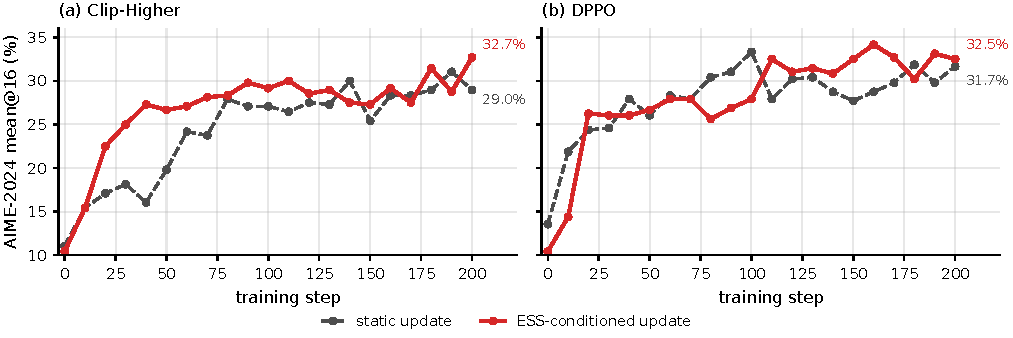
\includegraphics[width=0.8\linewidth]{figures_mains/result/8b/curves/overall.pdf}
  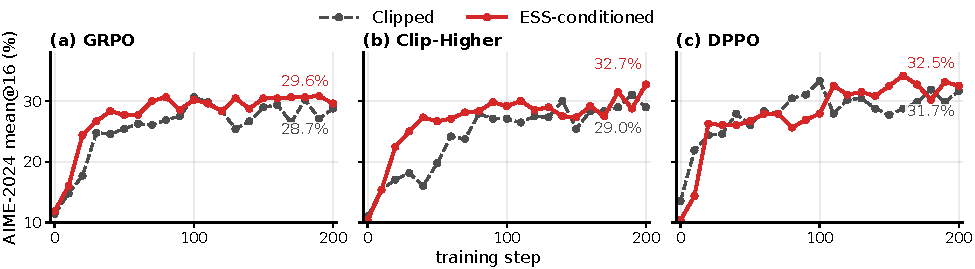
\includegraphics[width=\linewidth]
  {figures_mains/result/8b/curves/overall_with_dppo_compact.pdf}
  \caption{Qwen3-8B math RLVR over 200 policy updates. Dashed curves apply
  clipping throughout training, and solid curves use the ESS-conditioned
  counterpart. (a) GRPO. (b) Clip-Higher. (c) DPPO. End labels report the step-200
  AIME-2024 mean@16.}
  \label{fig:llm-8b-transfer}
\end{figure}

We then reduce the model to Qwen3-1.7B while retaining the mathematical-reasoning objective. Figure~\ref{fig:llm-17b-transfer} reports evaluation performance for the two matched learning-rate recipes and overlays ESS. ESS remains above the conditioning threshold of $0.1$, so the optimizer never activates clipping and thus behaves like TIS-3. Performance remains stable and improves even during the extended 500-step training run. This theoretical explanation is consistent with observations in other work, where TIS shows reasonable training trajectories.

\begin{wrapfigure}[12]{R}{0.4\textwidth}
  \vspace{-0.7\baselineskip}
  \centering
  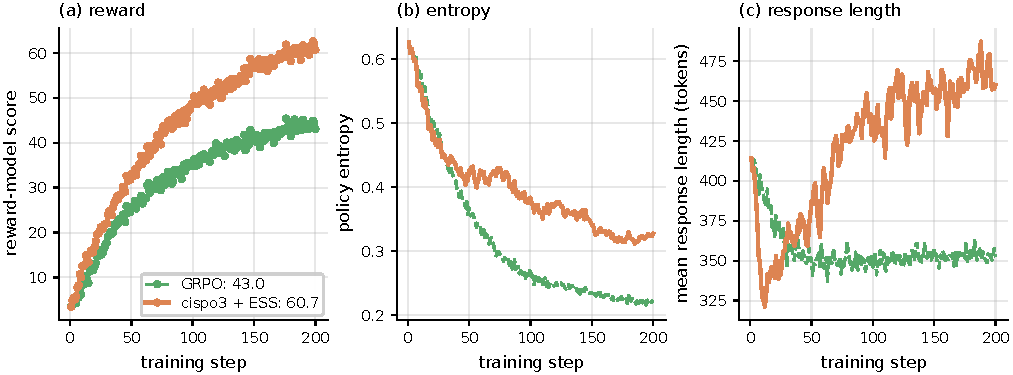
\includegraphics[width=0.8\linewidth]
  {figures_mains/result/rlhf_4b/overall.pdf}
  \caption{RLHF on Qwen3-4B-Instruct-2507. End labels report the step-200 observations.}
  \label{fig:llm-rlhf-transfer}
  \vspace{-0.6\baselineskip}
\end{wrapfigure}

\paragraph{Results on RLHF.}
We further change both the objective and the data by training
Qwen3-4B-Instruct-2507 on Anthropic HH-RLHF \citep{bai2022hh}, using
Skywork-Reward-Llama-3.1-8B \citep{liu2024skywork} as the reward model.
Figure~\ref{fig:llm-rlhf-transfer} shows the same advantage under
learned-reward optimization. The TIS-3-plus-ESS recipe reaches a final
reward-model score of $60.7$, compared with $43.0$ for GRPO. This experiment
evaluates optimization of the specified reward model rather than human
preference directly.


\subsection{Ablations}

The ESS-conditioned construction contains two distinct choices: the threshold
determines when the update changes, while the low-ESS rule determines how it changes. We study these components separately.

\paragraph{ESS threshold.}
Figure~\ref{fig:ess-threshold-ablation} varies only $\tau$ in the TIS-3/GRPO construction. Thresholds $0.05$, $0.1$, and $0.2$ all avoid the collapse of ungated TIS-3, with last-observed AIME scores of $43.1\%$,
$38.5\%$, and $34.8\%$, respectively, demonstrating that the collapse-prevention behavior persists across the tested range.

\paragraph{Clipping versus skipping.}
ESS determines when to intervene but does not prescribe the intervention itself. We therefore replace clipping with a complete update veto while keeping the same ESS threshold.

Figure~\ref{fig:skip-variants} isolates a complete update veto on the unclipped branch. Skipping raises the final score only slightly, from $34.6\%$
to $35.6\%$, while reducing the peak from $44.4\%$ to $35.6\%$. By contrast,
ESS-conditioned clipping in Figure~\ref{fig:llm-noclip-gate}(d) reaches a
$43.3\%$ peak and retains $38.1\%$. The intervention must therefore preserve
useful gradient signal after ESS identifies an unreliable minibatch.


%Together, the ablations separate the two roles in ESS-conditionedoptimization. The ESS threshold determines the intervention time; the post-threshold estimator determines the resulting bias--variation tradeoff. This distinction mirrors the theoretical analysis: identifying deteriorationin importance-weighted reliability does not by itself determine how the gradient estimator should be modified.


\section{Conclusion}

We studied a finite-sample perspective on policy optimization that provides a theoretical foundation for finite-sample policy improvement. Off-policy gradients admit an importance-weighted mean-estimation formulation, under which ESS enters directly through the second moment of the importance weights. Our theory connects this finite-sample estimation error to policy improvement and separately characterizes when clipping compensates for the gradient alignment it removes. We demonstrated our theoretical analysis through two empirical analyses, one in a Gaussian bandit and one in large language models. We then extended our analysis to a simple reliability-aware optimization method, which prevents the collapse seen with the previous updates and demonstrates strong empirical performance across model sizes and objectives.


\bibliographystyle{plainnat}
\bibliography{references}



\appendix

\section{Details for Gaussian Bandit Experiments}
\label{app:gaussian}

This section provides the experimental setup and exact calculations underlying the Gaussian bandit experiments in Section~\ref{sec:gaussian-example}. All estimator moments, mean-squared errors, and expected one-step gains are computed analytically using truncated Gaussian moments. Monte Carlo simulation is used only to evaluate the batch-level probabilities in Figure~\ref{fig:gaussian-policy-comparison}.

\subsection{Experimental setup}

\paragraph{Policy pair and ESS.}
We fix the current policy and consider a family of rollout policies
\[
P_\theta=\mathcal N(\theta,1),
\qquad
Q_\Delta=\mathcal N(\theta-\Delta,1),
\qquad
\Delta\ge0.
\]
Thus, $\Delta$ controls only the distance between the current and rollout policies. Defining the centered action $z:=a-\theta$, we have
\[
z\sim\mathcal N(0,1) \quad\text{under }P_\theta,
\qquad
z\sim\mathcal N(-\Delta,1) \quad\text{under }Q_\Delta.
\]
The corresponding likelihood ratio is
\[
W_\Delta(z)
=
\frac{dP_\theta}{dQ_\Delta}(z)
=
\exp\!\left\{\Delta z+\frac{\Delta^2}{2}\right\}.
\]
A direct calculation gives
\begin{equation}
\E_{Q_\Delta}[W_\Delta^2]=e^{\Delta^2},
\qquad
\rho(\Delta)=e^{-\Delta^2},
\qquad
\Delta=\sqrt{-\log\rho}.
\label{eq:gaussian-ratio-ess}
\end{equation}
Hence, $\Delta$ and ESS are in one-to-one correspondence. We therefore parameterize all figures by $\rho$, while carrying out the calculations using the corresponding value of $\Delta$.

\paragraph{Reward and policy-gradient contribution.}
We use the quadratic reward
\[
R(a)=-\frac12(a-a^\star)^2
\]
and define $d:=a^\star-\theta>0$. The current-policy objective and population gradient are
\[
J(\theta)=-\frac12(d^2+1),
\qquad
\nabla J(\theta)=d.
\]
Throughout the experiment, we hold $\theta$, and therefore $d$, fixed while varying $\Delta$.

Using the exact current-policy value as the baseline, the advantage for a centered action $z$ is
\[
A(z)=dz+\frac{1-z^2}{2}.
\]
Since the score of $\mathcal N(\theta,1)$ is $z$, the corresponding per-sample policy-gradient contribution is
\[
\psi(z):=zA(z)=dz^2+\frac{z-z^3}{2},
\qquad
\E_{P_\theta}[\psi(z)]=d.
\]

\paragraph{Estimators.}
Given samples
\[
z_1,\ldots,z_N\stackrel{\mathrm{iid}}{\sim}\mathcal N(-\Delta,1),
\]
we compare IS, TIS-3, and PPO. Their per-sample contributions are
\begin{align*}
\xi_{\mathrm{IS}}(z) &:= W_\Delta(z)\psi(z),\\
\xi_{\mathrm{T}}(z) &:= \min\{W_\Delta(z),c\}\psi(z),\\
\xi_{\mathrm{P}}(z) &:= W_\Delta(z)\psi(z)M_{\epsilon,\Delta}(z),
\end{align*}
where $c=3$, $\epsilon=0.2$, and
\[
M_{\epsilon,\Delta}(z)
=
\mathbf 1\{A(z)\ge0,\ W_\Delta(z)\le1+\epsilon\}
+
\mathbf 1\{A(z)<0,\ W_\Delta(z)\ge1-\epsilon\}.
\]
The corresponding batch estimator is
\[
\widehat g_u
=
\frac1N\sum_{i=1}^N\xi_u(z_i),
\qquad
u\in\{\mathrm{IS},\mathrm{T},\mathrm{P}\}.
\]

\subsection{Exact calculation of evaluation quantities}

All quantities reported in the Gaussian experiments, except for the batch-level probabilities, are computed exactly. For each estimator, define its first two per-sample moments by
\[
\mu_u(\Delta):=\E_{Q_\Delta}[\xi_u(z)],
\qquad
\nu_u(\Delta):=\E_{Q_\Delta}[\xi_u(z)^2].
\]
The corresponding batch moments and mean-squared error are
\begin{align*}
\E[\widehat g_u] &= \mu_u,\\
\E[\widehat g_u^2] &= \mu_u^2+\frac{\nu_u-\mu_u^2}{N},\\
\E[(\widehat g_u-d)^2] &= (\mu_u-d)^2+\frac{\nu_u-\mu_u^2}{N}.
\end{align*}
Thus, the pair $(\mu_u,\nu_u)$ determines both the gradient-estimation MSE and the second-moment term appearing in the policy-improvement certificate.

For IS, change of measure gives
\[
\mu_{\mathrm{IS}}=d,
\qquad
\nu_{\mathrm{IS}}
=
e^{\Delta^2}
\E_{V\sim\mathcal N(\Delta,1)}[\psi(V)^2].
\]
For PPO,
\begin{align*}
\mu_{\mathrm{P}}
&=
\E_{U\sim\mathcal N(0,1)}[\psi(U)M_{\epsilon,\Delta}(U)],\\
\nu_{\mathrm{P}}
&=
e^{\Delta^2}
\E_{V\sim\mathcal N(\Delta,1)}[\psi(V)^2M_{\epsilon,\Delta}(V)].
\end{align*}

For TIS-3, the truncation boundary obtained from $W_\Delta(z)=c$ is
\[
b_c(\Delta):=\frac{\log c-\Delta^2/2}{\Delta}.
\]
Splitting the integral at this boundary yields
\begin{align*}
\mu_{\mathrm{T}}
&=
\E_{U\sim\mathcal N(0,1)}[\psi(U)\mathbf 1\{U\le b_c\}]
+
c\,\E_{U\sim\mathcal N(-\Delta,1)}[\psi(U)\mathbf 1\{U>b_c\}],\\
\nu_{\mathrm{T}}
&=
e^{\Delta^2}\E_{V\sim\mathcal N(\Delta,1)}[\psi(V)^2\mathbf 1\{V\le b_c\}]
+
c^2\E_{V\sim\mathcal N(-\Delta,1)}[\psi(V)^2\mathbf 1\{V>b_c\}].
\end{align*}

These expectations have closed forms because $\psi$ is a cubic polynomial and all estimator boundaries are linear thresholds in $z$. In particular, the advantage changes sign at
\[
z=d\pm\sqrt{d^2+1},
\]
while the PPO ratio boundaries are
\[
b_\pm(\Delta)
=
\frac{\log(1\pm\epsilon)-\Delta^2/2}{\Delta}.
\]
The real line can therefore be partitioned at the two advantage roots and the two PPO ratio boundaries, with the mask remaining constant on each resulting interval.

For completeness, define the truncated standard-normal moments
\[
I_j(a,b):=\int_a^b z^j\phi(z)\,dz.
\]
They satisfy
\[
I_0(a,b)=\Phi(b)-\Phi(a),
\qquad
I_1(a,b)=\phi(a)-\phi(b),
\]
and, for $j\ge2$,
\[
I_j(a,b)
=
a^{j-1}\phi(a)-b^{j-1}\phi(b)+(j-1)I_{j-2}(a,b).
\]
After shifting the integration variable for nonzero Gaussian means, all moments above reduce to finite sums of these truncated Gaussian moments.

\subsection{ESS and IS reliability}

Figures~\ref{fig:gaussian-is-mse} and~\ref{fig:gaussian-policy-comparison} evaluate the ESS-dependent reliability result for the IS estimator. We set
\[
N=32,
\qquad
d=2,
\qquad
\delta=0.1.
\]

\paragraph{Exact MSE and theoretical envelope.}
Define
\[
M_2(\Delta)
:=
\rho(\Delta)\nu_{\mathrm{IS}}(\Delta)
=
\E_{V\sim\mathcal N(\Delta,1)}[\psi(V)^2].
\]
For $d=2$, this quantity is
\[
M_2(\Delta)
=
\frac{\Delta^6}{4}
-2\Delta^5
+\frac{29\Delta^4}{4}
-18\Delta^3
+\frac{65\Delta^2}{2}
-24\Delta
+\frac{29}{2}.
\]
Since IS is unbiased, its exact MSE and the finite-moment upper bound in Equation~\eqref{eq:rho-gradient-mse-bound} are
\begin{align*}
\operatorname{MSE}_{\mathrm{IS}}(\Delta)
&=
\frac1N\left\{\frac{M_2(\Delta)}{\rho(\Delta)}-d^2\right\},\\
\operatorname{MSE}_{\mathrm{IS}}(\Delta)
&\le
\frac{M_2(\Delta)}{N\rho(\Delta)}.
\end{align*}
Figure~\ref{fig:gaussian-is-mse} plots the exact MSE against $\rho=e^{-\Delta^2}$. No Monte Carlo approximation is used in this figure.

\paragraph{Batch-level improvement experiment.}
The left plot in Figure~\ref{fig:gaussian-policy-comparison} evaluates the corresponding batch-level policy-improvement statement. We consider 81 ESS values logarithmically spaced between $0.005$ and $0.9$. For each $\rho$, we set $\Delta=\sqrt{-\log\rho}$ and compute the theoretical error radius
\[
\varepsilon(\rho)
=
\sqrt{\frac{M_2(\Delta)}{\delta N\rho}}.
\]
At each ESS value, we independently generate $10^5$ batches of size $N$ from $Q_\Delta$ and compute
\[
\widehat g_{\mathrm{IS}}
=
\frac1N\sum_{i=1}^N W_\Delta(z_i)\psi(z_i).
\]
We then use the adaptive step from Theorem~\ref{thm:permissive-reliability},
\[
\gamma
=
\left(1-\frac{\varepsilon(\rho)}{|\widehat g_{\mathrm{IS}}|}\right)_+,
\]
where $L=1$. The theorem gives a positive certificate whenever
\[
|\widehat g_{\mathrm{IS}}|>\varepsilon(\rho).
\]
For the same batch, the exact change in the quadratic objective is
\[
\Delta J
=
d\gamma\widehat g_{\mathrm{IS}}
-
\frac{\gamma^2}{2}\widehat g_{\mathrm{IS}}^2.
\]
The figure reports the fraction of batches satisfying the positive-certificate condition and the fraction satisfying $\Delta J>0$. These correspond to the ``positive certificate'' and ``actual improvement'' curves, respectively.

As an additional check of the high-probability result, we record the event
\[
|\widehat g_{\mathrm{IS}}-d|\le\varepsilon(\rho).
\]
Across the displayed ESS grid, the minimum empirical coverage is $0.98277$, exceeding the required level $1-\delta=0.9$.

\subsection{Estimator crossover}

The center and right plots in Figure~\ref{fig:gaussian-policy-comparison} compare IS, TIS-3, and PPO under the common fixed step size $\eta=0.4$. For the quadratic objective, the smoothness inequality is exact: for any realized scalar update $h$,
\[
J(\theta+\eta h)-J(\theta)
=
\eta dh-\frac{\eta^2}{2}h^2.
\]
Taking expectation with $h=\widehat g_u$ gives
\begin{equation}
\mathcal G_u(\eta)
:=
\E[J(\theta+\eta\widehat g_u)-J(\theta)]
=
\eta d\mu_u
-
\frac{\eta^2}{2}
\left(\mu_u^2+\frac{\nu_u-\mu_u^2}{N}\right).
\label{eq:gaussian-exact-gain}
\end{equation}
Hence, the fixed-step certificate in Theorem~\ref{thm:fixed-step-certificate} coincides with the exact expected one-step improvement in this experiment.

\paragraph{Crossover criterion.}
The center plot shows
\[
\mathcal G_{\mathrm{T}}(\eta)-\mathcal G_{\mathrm{IS}}(\eta)
\qquad\text{and}\qquad
\mathcal G_{\mathrm{P}}(\eta)-\mathcal G_{\mathrm{IS}}(\eta)
\]
against ESS. Positive values indicate that the corresponding modified estimator yields larger expected one-step improvement than IS.

These gain differences are exactly equivalent to the crossover criterion in Corollary~\ref{cor:certificate-crossover}. Define
\[
S_u:=\E[\widehat g_u^2],
\qquad
m_u:=\E[(\widehat g_u-d)^2].
\]
Since $L=1$,
\begin{equation}
\{m_{\mathrm{IS}}-m_u\}
-
(1-\eta)\{S_{\mathrm{IS}}-S_u\}
=
\frac{2}{\eta}
\left\{\mathcal G_u(\eta)-\mathcal G_{\mathrm{IS}}(\eta)\right\}.
\label{eq:gaussian-crossover-identity}
\end{equation}
Therefore, the zero crossings in the center plot of Figure~\ref{fig:gaussian-policy-comparison} are precisely the estimator crossovers predicted by the corollary.

Using the exact moments above, the resulting crossover ESS values are
\[
\rho_{\mathrm{IS,TIS3}}=0.105,
\qquad
\rho_{\mathrm{IS,PPO}}=0.0392.
\]
The right plot gives the exact gains $\mathcal G_{\mathrm{IS}}$, $\mathcal G_{\mathrm{T}}$, and $\mathcal G_{\mathrm{P}}$ in the neighborhood of these two crossover points. The vertical lines and open markers indicate the corresponding roots.

TIS-3 has the smallest gradient MSE throughout the displayed ESS range, but this does not make it the preferred update everywhere. At high ESS, IS retains the larger expected gain. TIS-3 overtakes IS only once $\rho$ falls below $0.105$, while PPO crosses IS later at $\rho=0.0392$ and remains below TIS-3 throughout the displayed range. The experiment therefore illustrates the distinction established by the theory: estimator accuracy and policy improvement need not induce the same ordering.

\section{Details for LLM optimizations}
\label{app:llm-diagnostics}
In this section, we provide additional details on the experimental setup and
report supplementary ablation studies.

\subsection{Experimental Details}

Most experiments are conducted using NVIDIA A100 and B200 GPUs. Our
implementation is built on VeRL~\citep{sheng2024verl}, with
Megatron~\citep{shoeybi2019megatron} used as the training backend and
vLLM~\citep{kwon2023efficient} used for efficient rollout generation.
The main training configurations are summarized in Table~\ref{tab:hyperparameters}.

\begin{table}[t]
    \centering
    \caption{Hyperparameters used in our experiments.}
    \label{tab:hyperparameters}
    \small
    \begin{tabular}{lccc}
        \toprule
        \textbf{Hyperparameters}
        & \textbf{Qwen3-8B-Base}
        & \textbf{Qwen3-30B-A3B-Base}
        & \textbf{Qwen3-1.7B-Base} \\
        \midrule
        Learning Rate       & $10^{-6}$ & $10^{-6}$ & $10^{-6}$ \\
        PPO Epochs           & 1         & 1         & 1         \\
        Max Prompt Length    & 2048      & 2048      & 2048      \\
        Max Response Length  & 8192      & 8192      & 8192      \\
        Train Batch Size     & 256       & 256       & 64        \\
        PPO Mini Batch Size  & 32        & 32        & 16        \\
        Rollout Temperature  & 1.0       & 1.0       & 1.0       \\
        \bottomrule
    \end{tabular}
\end{table}

For evaluation, we periodically assess each method throughout RL training on
AIME24. We run evaluations every 10 training steps for all model scales. To
ensure consistent comparisons across experiments, we use the same sampling
configuration throughout, with temperature $0.7$ and top-$p$ $0.95$.
\subsection{Additional Results}

\paragraph{Results on other benchmarks}

We show the results on other benchmark datasets.


\paragraph{ESS threshold.}
Figure~\ref{fig:ess-threshold-ablation} varies only $\tau$ in the
TIS-3/GRPO construction. Thresholds $0.05$, $0.1$, and $0.2$ all avoid the
collapse of ungated TIS-3, with last-observed AIME scores of $43.1\%$,
$38.5\%$, and $34.8\%$, respectively. The threshold therefore controls the
timing of clipping, and the resulting performance varies with how long TIS-3
remains active. The collapse-prevention behavior persists across the tested
range.

\begin{figure}[htbp]
  \centering
  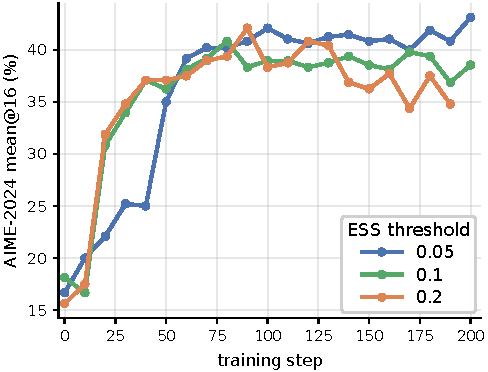
\includegraphics[width=0.52\linewidth]
  {figures_mains/result/q30ba3b/cispo3_ess_threshold/eval.pdf}
  \caption{Sensitivity to the ESS threshold for TIS-3 with GRPO clipping on
  Qwen3-30B-A3B. Curves use $\tau\in\{0.05,0.1,0.2\}$; clipping is activated
  when ESS falls below the corresponding threshold.}
  \label{fig:ess-threshold-ablation}
\end{figure}

\paragraph{Clipping versus skipping.}
ESS determines when to intervene but does not prescribe the intervention
itself. We therefore replace clipping with a complete update veto while
keeping the same ESS threshold.

Figure~\ref{fig:skip-variants} isolates a complete update veto on the
unclipped branch. Skipping raises the final score only slightly, from $34.6\%$
to $35.6\%$, while reducing the peak from $44.4\%$ to $35.6\%$. By contrast,
ESS-conditioned clipping in Figure~\ref{fig:llm-noclip-gate} reaches a
$43.3\%$ peak and retains $38.1\%$. The intervention must therefore preserve
useful gradient signal after ESS identifies an unreliable minibatch.

The separate TIS-5 comparison in Figure~\ref{fig:tis5-skip} shows the
complementary regime. Here skipping prevents complete collapse and raises the
final AIME score from $0.00\%$ to $39.4\%$. Together, the two comparisons
separate the timing decision supplied by ESS from the estimator choice made
after that transition.

\begin{figure}[htbp]
  \centering
  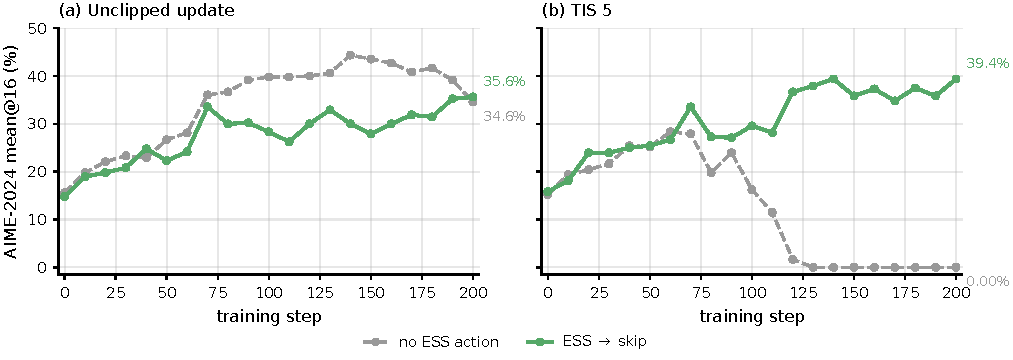
\includegraphics[width=0.52\linewidth]
  {figures_mains/result/q30ba3b/skip_gate/overall.pdf}
  \caption{ESS-conditioned update skipping on the unclipped
  Qwen3-30B-A3B trajectory. The dashed curve applies every update, and the
  solid curve skips the update when ESS falls below
  $0.1$. End labels report the final observed AIME-2024 mean@16.}
  \label{fig:skip-variants}
\end{figure}
\FloatBarrier

Together, the ablations separate the two roles in ESS-conditioned
optimization. The ESS threshold determines the intervention time; the
post-threshold estimator determines the resulting bias--variation tradeoff.
This distinction mirrors the theoretical analysis: identifying deterioration
in importance-weighted reliability does not by itself determine how the
gradient estimator should be modified.



\begin{figure}[htbp]
  \centering
  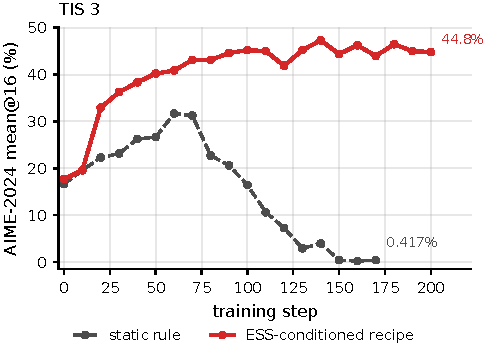
\includegraphics[width=0.54\linewidth]
  {figures_mains/result/q30ba3b/curves/tis3.pdf}
  \caption{Separated TIS-3 collapse comparison from the main 30B experiment.
  Ungated TIS-3 is shown against the ESS-conditioned Clip-Higher trajectory
  used in Figure~\ref{fig:llm-main}(b).}
  \label{fig:llm-tis3-collapse}
\end{figure}

\begin{figure}[htbp]
  \centering
  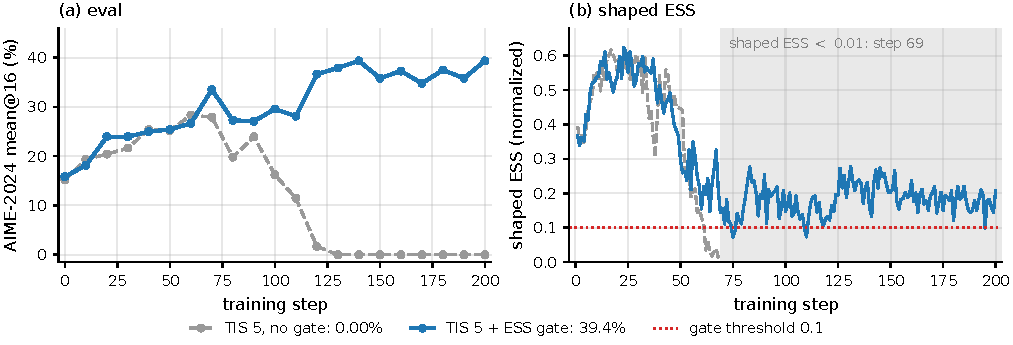
\includegraphics[width=0.54\linewidth]
  {figures_mains/result/q30ba3b/tis5/overall.pdf}
  \caption{Separated TIS-5 skipping comparison on Qwen3-30B-A3B. The dashed
  curve continues TIS-5 throughout training; the solid curve skips low-ESS
  updates.}
  \label{fig:tis5-skip}
\end{figure}


\subsection{Additional results on training dynamics}

The main text reports evaluation performance. We record here how often the
conditional rule intervenes and the accompanying training dynamics.

\begin{figure}[htbp]
  \centering
  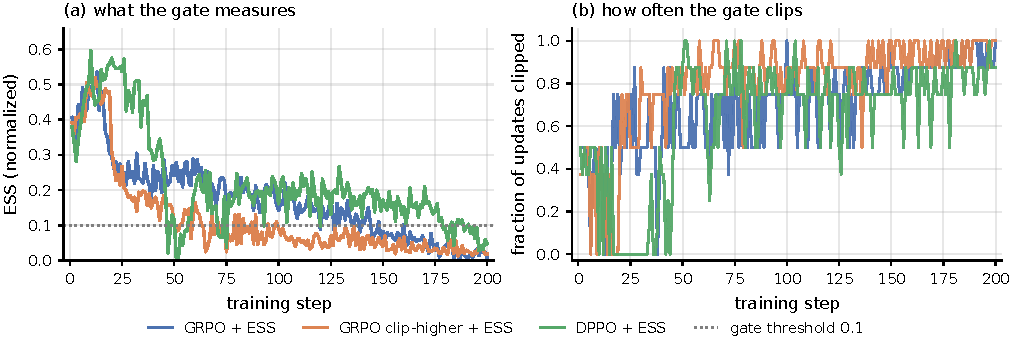
\includegraphics[width=\linewidth]{figures_mains/result/q30ba3b/gate/overall.pdf}
  \caption{Realized ESS-conditioned intervention schedules. Each panel pairs
  the per-step intervention fraction (thin black) and its trailing seven-step
  mean (thick black) with ESS (red). GRPO and DPPO use raw ESS;
  Clip-Higher uses shaped ESS after the coefficient cap. The dotted line marks
  the threshold $0.1$.}
  \label{fig:llm-gate-action}
\end{figure}

Figure~\ref{fig:llm-gate-action} shows the intended temporal ordering:
intervention is already possible early, but its frequency increases as ESS
contracts. The remaining figures record response length, entropy, and reward
diagnostics.

\begin{figure}[htbp]
  \centering
  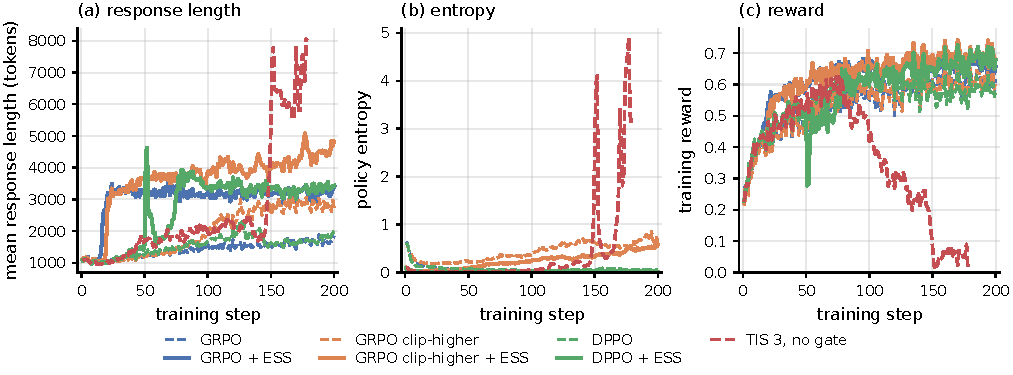
\includegraphics[width=\linewidth]{figures_mains/result/q30ba3b/dynamics/overall.pdf}
  \caption{Training dynamics for the main comparisons. The static TIS 3 run
  develops extreme response length and entropy together with a collapse in
  training reward. The safeguards and their ESS-conditional variants avoid
  this failure over the reported 200 steps.}
  \label{fig:llm-dynamics}
\end{figure}

\section{Proofs for the theoretical results}
\label{app:proofs}

At update $k$, all expectations and probabilities below are conditional on the
preceding updates. The current policy is therefore fixed, and the rollout
samples used at update $k$ are independent draws from $Q$. We suppress this
conditioning throughout.


To separate likelihood-ratio dispersion from the scale of the associated
gradient contributions, define
\begin{equation}
 M_{2,k}
 :=
 \frac{\E_Q[W_k^2\|f_k\|_2^2]}
      {\E_Q[W_k^2]}
 =
 \rho_k\E_Q[W_k^2\|f_k\|_2^2].
 \label{eq:weighted-contribution-scale}
\end{equation}
Since $\E_Q[W_k^2]=\rho_k^{-1}$ and
$\E[\widehat g_k]=g_k$, the exact IS MSE is
\begin{equation}
 \E\|\widehat g_k-g_k\|_2^2
 =
 \frac1N
 \left(
 \frac{M_{2,k}}{\rho_k}
 -
 \|g_k\|_2^2
 \right)
 \le
 \frac{M_{2,k}}{N\rho_k}.
 \label{eq:rho-gradient-mse}
\end{equation}

Equation~\eqref{eq:rho-gradient-mse} isolates the role of ESS in the
finite-sample error. The factor $\rho_k^{-1}$ captures concentration of the
importance weights, while $M_{2,k}$ captures the magnitude of the gradient
contributions under the corresponding squared-weight tilt. For fixed
$M_{2,k}$, the IS MSE therefore increases monotonically with
$\rho_k^{-1}$. If $f_k$ is bounded, then
$M_{2,k}\le\|f_k\|_\infty^2$, recovering the standard bounded-contribution
specialization.



\subsection{IS identity and exact mean-square error}

We first verify the unbiasedness and mean-square calculation used in
Section~\ref{sec:gradient-reliability}. Recall that
\[
 f_k
 =
 (R-b(X))
 \nabla_\theta\log P_{\theta_k}(Y\mid X),
 \qquad
 W_k
 =
 \frac{dP_{\theta_k}}{dQ}.
\]
By change of measure,
\begin{align*}
 \E_Q[W_kf_k]
 &=
 \E_{P_{\theta_k}}
 \left[
 (R-b(X))
 \nabla_\theta\log P_{\theta_k}(Y\mid X)
 \right].
\end{align*}
The baseline term vanishes after conditioning on $X$, since
\begin{align*}
 &\E_{P_{\theta_k}}
 \left[
 b(X)\nabla_\theta\log P_{\theta_k}(Y\mid X)
 \,\middle|\,X
 \right]\\
 &\qquad=
 b(X)
 \int
 P_{\theta_k}(y\mid X)
 \nabla_\theta\log P_{\theta_k}(y\mid X)
 \,d\lambda(y)\\
 &\qquad=
 b(X)\nabla_\theta
 \int P_{\theta_k}(y\mid X)\,d\lambda(y)
 =0.
\end{align*}
The remaining term is the score-function identity, and hence
\[
 \E_Q[W_kf_k]
 =
 \nabla J(\theta_k)
 =
 g_k.
\]
Consequently,
$\E[\widehat g_k]=g_k$.

To compute the MSE, let
\[
 \xi_i:=W_{k,i}f_{k,i}-g_k.
\]
Then $\E[\xi_i]=0$ and
\[
 \widehat g_k-g_k
 =
 \frac1N\sum_{i=1}^N\xi_i.
\]
Independence eliminates the cross terms, giving
\begin{align*}
 \E\|\widehat g_k-g_k\|_2^2
 &=
 \frac1N
 \E_Q\|W_kf_k-g_k\|_2^2\\
 &=
 \frac1N
 \left\{
 \E_Q[W_k^2\|f_k\|_2^2]
 -
 \|g_k\|_2^2
 \right\}.
\end{align*}
Since
\[
 \E_Q[W_k^2]
 =
 \rho_k^{-1},
 \qquad
 M_{2,k}
 =
 \rho_k\E_Q[W_k^2\|f_k\|_2^2],
\]
we obtain
\[
 \E\|\widehat g_k-g_k\|_2^2
 =
 \frac1N
 \left(
 \frac{M_{2,k}}{\rho_k}
 -
 \|g_k\|_2^2
 \right)
 \le
 \frac{M_{2,k}}{N\rho_k},
\]
which proves Equation~\eqref{eq:rho-gradient-mse}.


\subsection{Proof of Lemma~\ref{lem:gradient-error-progress}}

Suppose
$\|\widehat g-g\|_2\le\varepsilon$.
By $L$-smoothness, for every $\gamma\ge0$,
\[
 J(\theta+\gamma\widehat g)-J(\theta)
 \ge
 \gamma g^\top\widehat g
 -
 \frac{L\gamma^2}{2}
 \|\widehat g\|_2^2.
\]
Moreover,
\begin{align*}
 g^\top\widehat g
 &=
 \|\widehat g\|_2^2
 +(g-\widehat g)^\top\widehat g\\
 &\ge
 \|\widehat g\|_2^2
 -
 \|g-\widehat g\|_2\|\widehat g\|_2\\
 &\ge
 \|\widehat g\|_2
 \left(
 \|\widehat g\|_2-\varepsilon
 \right).
\end{align*}
Therefore
\[
 J(\theta+\gamma\widehat g)-J(\theta)
 \ge
 \gamma\|\widehat g\|_2
 \left(
 \|\widehat g\|_2-\varepsilon
 \right)
 -
 \frac{L\gamma^2}{2}\|\widehat g\|_2^2.
\]
For $\widehat g\neq0$, the right-hand side is a concave quadratic in
$\gamma$, whose nonnegative maximizer is
\[
 \gamma
 =
 \frac1L
 \left(
 1-\frac{\varepsilon}{\|\widehat g\|_2}
 \right)_+.
\]
Substitution yields
\[
 J(\theta+\gamma\widehat g)-J(\theta)
 \ge
 \frac1{2L}
 \left(
 \|\widehat g\|_2-\varepsilon
 \right)_+^2.
\]
When $\widehat g=0$, both the chosen step and the claimed lower bound are zero.
This proves Lemma~\ref{lem:gradient-error-progress}.


\subsection{Proof of Lemma~\ref{lem:rho-gradient-reliability}}

If $M_{2,k}=0$, Equation~\eqref{eq:rho-gradient-mse} makes the result
immediate. Otherwise, Markov's inequality applied to
$\|\widehat g_k-g_k\|_2^2$ gives
\begin{align*}
 &\Pr\left(
 \|\widehat g_k-g_k\|_2
 >
 \sqrt{\frac{M_{2,k}}{\delta N\rho_k}}
 \right)\\
 &\qquad\le
 \frac{
 \E\|\widehat g_k-g_k\|_2^2
 }{
 M_{2,k}/(\delta N\rho_k)
 }
 \le
 \delta,
\end{align*}
where the last inequality follows from
Equation~\eqref{eq:rho-gradient-mse}. Taking complements proves
Equation~\eqref{eq:rho-gradient-concentration}.


\subsection{Proof of Theorem~\ref{thm:permissive-reliability}}

By Lemma~\ref{lem:rho-gradient-reliability}, the event
\[
 \|\widehat g_k-g_k\|_2
 \le
 \varepsilon_k(\delta)
 :=
 \sqrt{\frac{M_{2,k}}{\delta N\rho_k}}
\]
has probability at least $1-\delta$.
On this event, Lemma~\ref{lem:gradient-error-progress} applies with
$\theta=\theta_k$, $\widehat g=\widehat g_k$,
$\varepsilon=\varepsilon_k(\delta)$, and $L=L_k$.
Using the step in Equation~\eqref{eq:is-safe-step} gives
Equation~\eqref{eq:permissive-reliability}.


\subsection{Proof of Corollary~\ref{cor:positive-improvement-probability}}


Theorem~\ref{thm:permissive-reliability} makes the optimization consequence of ESS explicit. Define the positive-certificate event as
\begin{equation}
 \mathcal C_k
 :=
 \left\{
 \|\widehat g_k\|_2>\varepsilon_k(\delta)
 \right\}.
 \label{eq:positive-is-certificate}
\end{equation}
Decreasing ESS enlarges the error radius and therefore makes this condition harder to satisfy. The same argument also controls the probability of obtaining an improving
update. 
\begin{corollary}[Positive certificate and actual improvement]
\label{cor:positive-improvement-probability}
Under the update of
Theorem~\ref{thm:permissive-reliability},
\begin{equation}
 \Pr(\mathcal C_k)-\delta
 \le
 \Pr\!\lbrace
 J(\theta_k+\gamma_k\widehat g_k)>J(\theta_k)
 \rbrace
 \le
 \Pr(\mathcal C_k).
 \label{eq:positive-improvement-probability}
\end{equation}
\end{corollary}

The upper bound follows because $\gamma_k=0$ whenever
$\mathcal C_k$ does not occur. On the reliability event of
Lemma~\ref{lem:rho-gradient-reliability}, every batch in $\mathcal C_k$
satisfies the strictly positive lower bound in
Theorem~\ref{thm:permissive-reliability}; the complement of this reliability
event has probability at most $\delta$, giving the lower bound.


Let
\[
 \mathcal R_k
 :=
 \left\{
 \|\widehat g_k-g_k\|_2
 \le
 \varepsilon_k(\delta)
 \right\}
\]
be the reliability event and recall
\[
 \mathcal C_k
 :=
 \left\{
 \|\widehat g_k\|_2>\varepsilon_k(\delta)
 \right\}.
\]
Lemma~\ref{lem:rho-gradient-reliability} gives
$\Pr(\mathcal R_k)\ge1-\delta$.

On $\mathcal C_k\cap\mathcal R_k$, the lower bound in
Theorem~\ref{thm:permissive-reliability} is strictly positive. Hence
\begin{align*}
 \Pr\!\left(
 J(\theta_k+\gamma_k\widehat g_k)>J(\theta_k)
 \right)
 &\ge
 \Pr(\mathcal C_k\cap\mathcal R_k)\\
 &\ge
 \Pr(\mathcal C_k)-\Pr(\mathcal R_k^c)\\
 &\ge
 \Pr(\mathcal C_k)-\delta.
\end{align*}
Conversely, if $\mathcal C_k$ does not occur, then
$\gamma_k=0$ by Equation~\eqref{eq:is-safe-step}; strict improvement is
therefore impossible. Thus
\[
 \Pr\!\left(
 J(\theta_k+\gamma_k\widehat g_k)>J(\theta_k)
 \right)
 \le
 \Pr(\mathcal C_k),
\]
which proves Corollary~\ref{cor:positive-improvement-probability}.

\subsubsection{Proof of Lemma~\ref{lem:general-mse-reliability}}

Apply Markov's inequality to the nonnegative random variable
$\|\widehat g_k(u)-g_k\|_2^2$:
\[
 \Pr\left(
 \|\widehat g_k(u)-g_k\|_2
 >
 \sqrt{\frac{m_k(u)}{\delta}}
 \right)
 \le
 \frac{
 \E\|\widehat g_k(u)-g_k\|_2^2
 }{
 m_k(u)/\delta
 }
 =
 \delta.
\]
Taking complements proves
Equation~\eqref{eq:general-mse-reliability}.


\subsubsection{Proof of Theorem~\ref{thm:fixed-step-certificate}}

For any realization of $\widehat g_k(u)$, $L_k$-smoothness gives
\[
 J(\theta_k+\eta_k\widehat g_k(u))-J(\theta_k)
 \ge
 \eta_k g_k^\top\widehat g_k(u)
 -
 \frac{L_k\eta_k^2}{2}
 \|\widehat g_k(u)\|_2^2.
\]
Taking expectations yields
\[
 \E\!\left[
 J(\theta_k+\eta_k\widehat g_k(u))-J(\theta_k)
 \right]
 \ge
 \eta_k g_k^\top\E[\widehat g_k(u)]
 -
 \frac{L_k\eta_k^2}{2}
 \E\|\widehat g_k(u)\|_2^2.
\]

It remains to express the right-hand side through the estimator MSE.
Expanding $m_k(u)$ gives
\[
 m_k(u)
 =
 \E\|\widehat g_k(u)\|_2^2
 -
 2g_k^\top\E[\widehat g_k(u)]
 +
 \|g_k\|_2^2,
\]
and hence
\[
 2g_k^\top\E[\widehat g_k(u)]
 =
 \|g_k\|_2^2
 +
 \E\|\widehat g_k(u)\|_2^2
 -
 m_k(u).
\]
Substituting this identity into the smoothness bound gives
\[
 B_k(u;\eta_k)
 =
 \frac{\eta_k}{2}\|g_k\|_2^2
 -
 \frac{\eta_k}{2}m_k(u)
 +
 \frac{\eta_k}{2}(1-L_k\eta_k)
 \E\|\widehat g_k(u)\|_2^2,
\]
which is Equation~\eqref{eq:certificate-mse-form} and proves the theorem.


\subsubsection{Proof of Corollary~\ref{cor:certificate-crossover}}

Apply Equation~\eqref{eq:certificate-mse-form} to $u$ and $v$. The common
term $\eta_k\|g_k\|_2^2/2$ cancels, giving
\begin{align*}
 B_k(u;\eta_k)-B_k(v;\eta_k)
 &=
 \frac{\eta_k}{2}
 \{m_k(v)-m_k(u)\}\\
 &\quad-
 \frac{\eta_k}{2}(1-L_k\eta_k)
 \left\{
 \E\|\widehat g_k(v)\|_2^2
 -
 \E\|\widehat g_k(u)\|_2^2
 \right\}.
\end{align*}
Since $\eta_k>0$, this difference is positive exactly under
Equation~\eqref{eq:general-estimator-crossover}.


\subsubsection{Proof of Proposition~\ref{prop:ess-estimator-crossover}}

Set $v=u_{\mathrm{IS}}$ in
Corollary~\ref{cor:certificate-crossover}. From
Equation~\eqref{eq:rho-gradient-mse},
\[
 m_k(u_{\mathrm{IS}})
 =
 \frac1N
 \left(
 \frac{M_{2,k}}{\rho_k}
 -
 \|g_k\|_2^2
 \right).
\]
Since IS is unbiased,
\[
 m_k(u_{\mathrm{IS}})
 =
 \E\|\widehat g_k(u_{\mathrm{IS}})\|_2^2
 -
 \|g_k\|_2^2,
\]
so
\[
 \E\|\widehat g_k(u_{\mathrm{IS}})\|_2^2
 =
 \frac{M_{2,k}}{N\rho_k}
 +
 \left(1-\frac1N\right)\|g_k\|_2^2.
\]
Substituting these two identities into
Equation~\eqref{eq:general-estimator-crossover} gives exactly
Equation~\eqref{eq:ess-estimator-crossover}.


\subsubsection{Proof of Proposition~\ref{prop:tis-close}}

For notational brevity, write
\[
 \widehat g_c
 :=
 \widehat g_k(u_{\mathrm T}^{(c)}),
 \qquad
 \widehat g_\infty
 :=
 \widehat g_k(u_{\mathrm T}^{(\infty)}).
\]
Their difference is
\[
 \widehat g_\infty-\widehat g_c
 =
 \frac1N\sum_{i=1}^N D_i,
 \qquad
 D_i
 :=
 A_i\sum_{t=1}^T
 (r_{i,t}-c)_+\ell_{i,t}.
\]

Let $H_c<\infty$ uniformly bound the conditional second moments in the
statement of the proposition. Using
$\|\sum_{t=1}^T x_t\|_2^2\le
T\sum_{t=1}^T\|x_t\|_2^2$,
\begin{align*}
 \E\|D_i\|_2^2
 &\le
 T\sum_{t=1}^T
 \E\left[
 \|A_i(r_{i,t}-c)_+\ell_{i,t}\|_2^2
 \right]\\
 &\le
 T H_c^2
 \sum_{t=1}^T
 \Pr(r_{i,t}>c)\\
 &=
 T^2H_c^2p_{c,k}.
\end{align*}
Jensen's inequality then gives
\[
 \E\|\widehat g_\infty-\widehat g_c\|_2^2
 \le
 T^2H_c^2p_{c,k}
 =
 O(p_{c,k}).
\]

To transfer this estimator bound to the policy-improvement certificate, use
the equivalent smoothness representation derived in the proof of
Theorem~\ref{thm:fixed-step-certificate}:
\[
 B_k(u;\eta_k)
 =
 \eta_k g_k^\top\E[\widehat g_k(u)]
 -
 \frac{L_k\eta_k^2}{2}
 \E\|\widehat g_k(u)\|_2^2.
\]
Let
$d_c:=\widehat g_\infty-\widehat g_c$.
Then
\begin{align*}
 B_k(u_{\mathrm T};\eta_k)
 -
 B_k(u_{\mathrm T}^{(\infty)};\eta_k)
 &=
 -\eta_k g_k^\top\E[d_c]\\
 &\quad+
 L_k\eta_k^2
 \E[\widehat g_\infty^\top d_c]
 -
 \frac{L_k\eta_k^2}{2}
 \E\|d_c\|_2^2.
\end{align*}
By Cauchy--Schwarz,
\begin{align*}
 \left|
 B_k(u_{\mathrm T};\eta_k)
 -
 B_k(u_{\mathrm T}^{(\infty)};\eta_k)
 \right|
 &\le
 \eta_k\|g_k\|_2
 \sqrt{\E\|d_c\|_2^2}\\
 &\quad+
 L_k\eta_k^2
 \sqrt{
 \E\|\widehat g_\infty\|_2^2
 \E\|d_c\|_2^2
 }\\
 &\quad+
 \frac{L_k\eta_k^2}{2}
 \E\|d_c\|_2^2.
\end{align*}
The first estimator bound shows that
$\E\|d_c\|_2^2=O(p_{c,k})$. With the remaining moments fixed, the first two
terms are therefore $O(\sqrt{p_{c,k}})$ and the last is $O(p_{c,k})$.
Hence
\[
 \left|
 B_k(u_{\mathrm T};\eta_k)
 -
 B_k(u_{\mathrm T}^{(\infty)};\eta_k)
 \right|
 =
 O(\sqrt{p_{c,k}}),
\]
as claimed.


\subsection{Additional specializations}

\paragraph{Intact prompt groups.}
Suppose $M$ prompts are independent and each prompt has $G$ conditionally
independent responses. Keep each prompt group intact and define
\[
 \Xi_{k,i}
 :=
 \frac1G\sum_{j=1}^G W_{k,ij}f_{k,ij}.
\]
A leave-one-out baseline is admissible because it excludes the focal response;
conditional on the prompt and the remaining responses, the focal score still
has mean zero. Hence
$\E[\Xi_{k,i}]=g_k$.

Jensen's inequality gives
\[
 \|\Xi_{k,i}\|_2^2
 \le
 \frac1G
 \sum_{j=1}^G
 W_{k,ij}^2\|f_{k,ij}\|_2^2.
\]
Repeating the sample-mean argument across the $M$ independent prompt groups
therefore yields, under bounded contributions,
\[
 \E\left\|
 \frac1M\sum_{i=1}^M\Xi_{k,i}-g_k
 \right\|_2^2
 \le
 \frac{\|f_k\|_\infty^2}{M\rho_k}.
\]
Applying Markov's inequality gives the corresponding version of
Lemma~\ref{lem:rho-gradient-reliability} with the number of independent
prompts $M$ in place of the number of responses $N$.

\paragraph{Bounded-contribution specialization.}
If $\|f_k\|_\infty<\infty$, then
\[
 M_{2,k}
 =
 \rho_k\E_Q[W_k^2\|f_k\|_2^2]
 \le
 \|f_k\|_\infty^2.
\]
Lemma~\ref{lem:rho-gradient-reliability} therefore reduces to the familiar
radius
\[
 \frac{\|f_k\|_\infty}
 {\sqrt{\delta N\rho_k}}.
\]


\end{document}
